\documentclass[11pt, spanish]{article}
\usepackage[spanish]{babel}
\selectlanguage{spanish}
\usepackage{natbib}
\usepackage{url}
\usepackage[utf8x]{inputenc}
\usepackage{graphicx}
\graphicspath{{images/}}
\usepackage{parskip}
\usepackage{fancyhdr}
\usepackage{vmargin}
\usepackage{multirow}
\usepackage{float}
\usepackage{chngpage}

\usepackage{subcaption}

\usepackage{hyperref}
\usepackage[
    type={CC},
    modifier={by-nc-sa},
    version={4.0},
]{doclicense}

\hypersetup{
    colorlinks=true,
    linkcolor=blue,
    filecolor=magenta,      
    urlcolor=cyan,
}

% para codigo
\usepackage{listings}
\usepackage{xcolor}



%% configuración de listings

\definecolor{listing-background}{HTML}{F7F7F7}
\definecolor{listing-rule}{HTML}{B3B2B3}
\definecolor{listing-numbers}{HTML}{B3B2B3}
\definecolor{listing-text-color}{HTML}{000000}
\definecolor{listing-keyword}{HTML}{435489}
\definecolor{listing-identifier}{HTML}{435489}
\definecolor{listing-string}{HTML}{00999A}
\definecolor{listing-comment}{HTML}{8E8E8E}
\definecolor{listing-javadoc-comment}{HTML}{006CA9}

\lstdefinestyle{eisvogel_listing_style}{
  language         = c++,
%$if(listings-disable-line-numbers)$
%  xleftmargin      = 0.6em,
%  framexleftmargin = 0.4em,
%$else$
  numbers          = left,
  xleftmargin      = 0em,
 framexleftmargin = 0em,
%$endif$
  backgroundcolor  = \color{listing-background},
  basicstyle       = \color{listing-text-color}\small\ttfamily{}\linespread{1.15}, % print whole listing small
  breaklines       = true,
  frame            = single,
  framesep         = 0.19em,
  rulecolor        = \color{listing-rule},
  frameround       = ffff,
  tabsize          = 4,
  numberstyle      = \color{listing-numbers},
  aboveskip        = 1.0em,
  belowskip        = 0.1em,
  abovecaptionskip = 0em,
  belowcaptionskip = 1.0em,
  keywordstyle     = \color{listing-keyword}\bfseries,
  classoffset      = 0,
  sensitive        = true,
  identifierstyle  = \color{listing-identifier},
  commentstyle     = \color{listing-comment},
  morecomment      = [s][\color{listing-javadoc-comment}]{/**}{*/},
  stringstyle      = \color{listing-string},
  showstringspaces = false,
  escapeinside     = {/*@}{@*/}, % Allow LaTeX inside these special comments
  literate         =
  {á}{{\'a}}1 {é}{{\'e}}1 {í}{{\'i}}1 {ó}{{\'o}}1 {ú}{{\'u}}1
  {Á}{{\'A}}1 {É}{{\'E}}1 {Í}{{\'I}}1 {Ó}{{\'O}}1 {Ú}{{\'U}}1
  {à}{{\`a}}1 {è}{{\'e}}1 {ì}{{\`i}}1 {ò}{{\`o}}1 {ù}{{\`u}}1
  {À}{{\`A}}1 {È}{{\'E}}1 {Ì}{{\`I}}1 {Ò}{{\`O}}1 {Ù}{{\`U}}1
  {ä}{{\"a}}1 {ë}{{\"e}}1 {ï}{{\"i}}1 {ö}{{\"o}}1 {ü}{{\"u}}1
  {Ä}{{\"A}}1 {Ë}{{\"E}}1 {Ï}{{\"I}}1 {Ö}{{\"O}}1 {Ü}{{\"U}}1
  {â}{{\^a}}1 {ê}{{\^e}}1 {î}{{\^i}}1 {ô}{{\^o}}1 {û}{{\^u}}1
  {Â}{{\^A}}1 {Ê}{{\^E}}1 {Î}{{\^I}}1 {Ô}{{\^O}}1 {Û}{{\^U}}1
  {œ}{{\oe}}1 {Œ}{{\OE}}1 {æ}{{\ae}}1 {Æ}{{\AE}}1 {ß}{{\ss}}1
  {ç}{{\c c}}1 {Ç}{{\c C}}1 {ø}{{\o}}1 {å}{{\r a}}1 {Å}{{\r A}}1
  {€}{{\EUR}}1 {£}{{\pounds}}1 {«}{{\guillemotleft}}1
  {»}{{\guillemotright}}1 {ñ}{{\~n}}1 {Ñ}{{\~N}}1 {¿}{{?`}}1
  {…}{{\ldots}}1 {≥}{{>=}}1 {≤}{{<=}}1 {„}{{\glqq}}1 {“}{{\grqq}}1
  {”}{{''}}1
}
\lstset{style=eisvogel_listing_style}


\usepackage[default]{sourcesanspro}

\setmarginsrb{2 cm}{1 cm}{2 cm}{2 cm}{1 cm}{1.5 cm}{1 cm}{1.5 cm}

\title{Práctica 2:\\
Satisfacción de restricciones  \hspace{0.05cm} }                           
\author{Antonio David Villegas Yeguas}                             
\date{\today}                                           


\makeatletter
\let\thetitle\@title
\let\theauthor\@author
\let\thedate\@date
\makeatother

\pagestyle{fancy}
\fancyhf{}
\rhead{\theauthor}
\lhead{\thetitle}
\cfoot{\thepage}

\begin{document}

%%%%%%%%%%%%%%%%%%%%%%%%%%%%%%%%%%%%%%%%%%%%%%%%%%%%%%%%%%%%%%%%%%%%%%%%%%%%%%%%%%%%%%%%%

\begin{titlepage}
    \centering
    \vspace*{0.3 cm}
    
\includegraphics[scale = 0.50]{ugr.png}\\[0.7 cm]
    %\textsc{\LARGE Universidad de Granada}\\[2.0 cm]   
    \textsc{\large 3º CSI 2019/20 - Grupo 1}\\[0.5 cm]            
    \textsc{\large Grado en Ingeniería Informática}\\[0.5 cm]              
    \rule{\linewidth}{0.2 mm} \\[0.2 cm]
    { \huge \bfseries \thetitle}\\
    \rule{\linewidth}{0.2 mm} \\[1 cm]
    
    \begin{minipage}{0.4\textwidth}
        \begin{flushleft} \large
            \emph{Autor:}\\
            \theauthor\\ 
			 \emph{DNI:}\\
            77021623-M
            \end{flushleft}
            \end{minipage}~
            \begin{minipage}{0.4\textwidth}
            \begin{flushright} \large
            \emph{Asignatura: \\
            Técnicas de los Sistemas Inteligentes}   \\     
            \emph{Correo:}\\
            advy99@correo.ugr.es           
        \end{flushright}
    \end{minipage}\\[0.5cm]
  
    {\large \thedate}\\[0.5cm]
    %{\url{https://github.com/advy99/TSI/}}
    {\doclicenseThis}
 	
    \vfill
    
\end{titlepage}

%%%%%%%%%%%%%%%%%%%%%%%%%%%%%%%%%%%%%%%%%%%%%%%%%%%%%%%%%%%%%%%%%%%%%%%%%%%%%%%%%%%%%%%%%

%\tableofcontents
%\pagebreak

%%%%%%%%%%%%%%%%%%%%%%%%%%%%%%%%%%%%%%%%%%%%%%%%%%%%%%%%%%%%%%%%%%%%%%%%%%%%%%%%%%%%%%%%%

\section{Introducción}

En esta práctica se nos propone resolver distintos problemas de satisfacción de restricciones. En cada problema, dado su enunciado, hay que decidir cuales son las variables que intervienen en el problema, el dominio que tienen dichas variables, y que restricciones tienen esas variables, como bien sabemos tras estudiar el tema 2 de la teoría de la asignatura.

Para resolver estos problemas propuestos usaremos la herramienta MiniZinc, un lenguaje de modelado de restricciones que cuenta con un IDE con el que podremos representar los problemas y resolverlos. Este lenguaje cuenta con distintas herramientas para resolver los problemas de satisfacción de restricciones (\textit{CSP solvers}), aunque para esta práctica solo utilizaremos Gecode, instalado por defecto.

\section{Ejercicio 1}

Puzzle Cripto-aritmético. El siguiente problema plantea un problema criptoaritmético, de forma que cada letra codifica un único dígito (es decir, un número entero en [0,9]) y cada dígito está asignado a una única letra. Se pide encontrar una asignación de dígitos a letras que satisfaga la siguiente suma:

\begin{lstlisting}
     TESTE
 +   FESTE
 +   DEINE
  =========
    KRAFTE
\end{lstlisting}

\subsection{Variables}

Tendremos 10 variables, una por letra. En MiniZinc lo representaremos con un array de 10 posiciones.

\subsection{Dominio de las variables}

Cada variable es un entero entre el número 0 y el 9 (ambos incluidos).

Usaremos variables auxiliares para gestionar los acarreos.

\subsection{Restricciones}

\textbf{1:} Cada variable tiene que tomar un valor distinto. Esto lo conseguiremos con el uso de la función \texttt{alldifferent(array)} de MiniZinc.

\textbf{2:} La suma de cada columna tiene que coincidir (con su respectivo acarreo). Usaremos 5 variables para almacenar el acarreo de cada suma, y haremos uso de \texttt{constraint} para hacer que las sumas sumando el acarreo (y dividido por 10, para que el resultado este entre 0..9) sean igual a la letra correspondiente. El acarreo será la misma operación, pero aplicando la operación módulo 10.


\subsection{Resultado}

\begin{figure}[H]
  \centering
      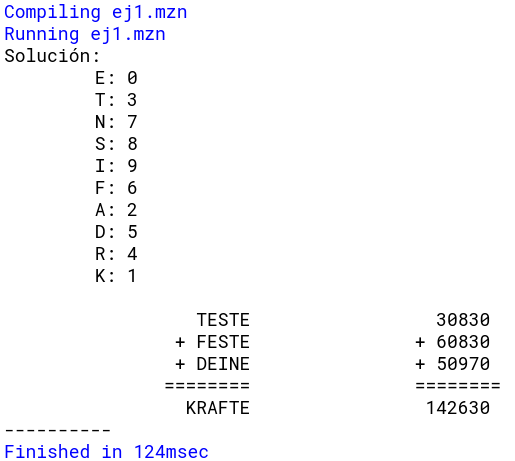
\includegraphics[scale = 0.30]{sol1.png}
 		 \caption{Solución obtenida para el ejercicio 1.}
  		\label{fig:ej1}

\end{figure}

\section{Ejercicio 2}
Encontrar un número X de 10 dígitos que satisfaga que el primer dígito de X representa el número de 0s en X, el segundo dígito de X representa el número de 1s en X, etc...

Por ejemplo, el número X=6210001000 satisface dicha condición.

\subsection{Variables}

Usaremos un array con 10 posiciones, de la 0 a la 9 (ambos incluidos) para representar el número X.

\subsection{Dominio de las variables}

Las variables son números enteros de 0 a 9.

\subsection{Restricciones}

El indice del dígito equivale al número de veces que aparece el dígito en el número X. Esto lo conseguimos en MiniZinc con un bucle, en el que para todo i desde 0 hasta 9, tiene que aparecer i veces.

\subsection{Resultado}

\begin{figure}[H]
  \centering
      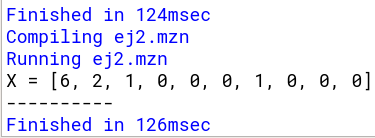
\includegraphics[scale = 0.50]{sol2.png}
 		 \caption{Solución obtenida para el ejercicio 2.}
  		\label{fig:ej2}

\end{figure}


\section{Ejercicio 3}

Encontrar una asignación de horarios que satisfaga las siguientes condiciones (condiciones en la sección de restricciones).

\subsection{Variables}

Usaremos un array con tantos elementos como profesores.

También usaremos una matriz con tantas filas como profesores y dos columnas, para representar el inicio y fin del horario de cada profesor.

\subsection{Dominio de las variables}

El array para la asignación de profesores puede tomar valores entre 9 y 14, las horas donde puede comenzar una clase, es decir, si, por ejemplo, toma el valor 9 en la posición 2, quiere decir que el profesor 2 da clase de 9:00 a 10:00.

La matriz puede tomar valores entre 9 y 15, el horario dado.

\subsection{Restricciones}

Las restricciones son que un aula solo puede estar ocupada por un profesor, esto lo hemos conseguido al usar una array con una posición por hora.

Otra restricción a tener en cuenta es que las clases son de 1 hora, luego no se repiten ningún profesor, usaremos \texttt{alldifferent(profesores)} para tener en cuenta esta restricción.

Cada profesor tiene un horario disponible. Esto lo solucionamos haciendo uso de la matriz de horarios, asegurando que la posición de un profesor en el array es mayor o igual que la hora de inicio y menor que la hora de fin (en la hora de fin menor estricto, ya que si un horario va de 9:00 a 13:00, no se puede dar clase a las 13:00 - 14:00).

\subsection{Resultado}


\begin{figure}[H]
  \centering
      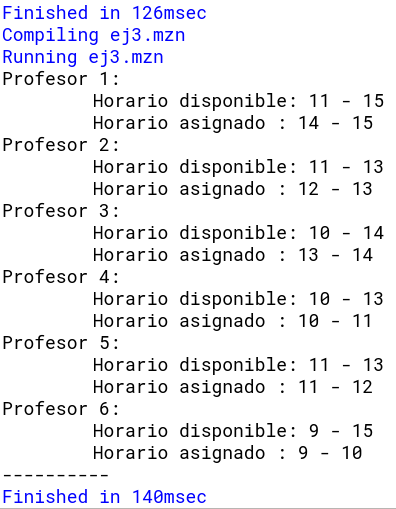
\includegraphics[scale = 0.30]{sol3.png}
 		 \caption{Solución obtenida para el ejercicio 3.}
  		\label{fig:ej3}

\end{figure}

\section{Ejercicio 4}


\subsection{Variables}

\subsection{Dominio de las variables}

\subsection{Restricciones}

\subsection{Resultado}


\begin{figure}[H]
  \centering
      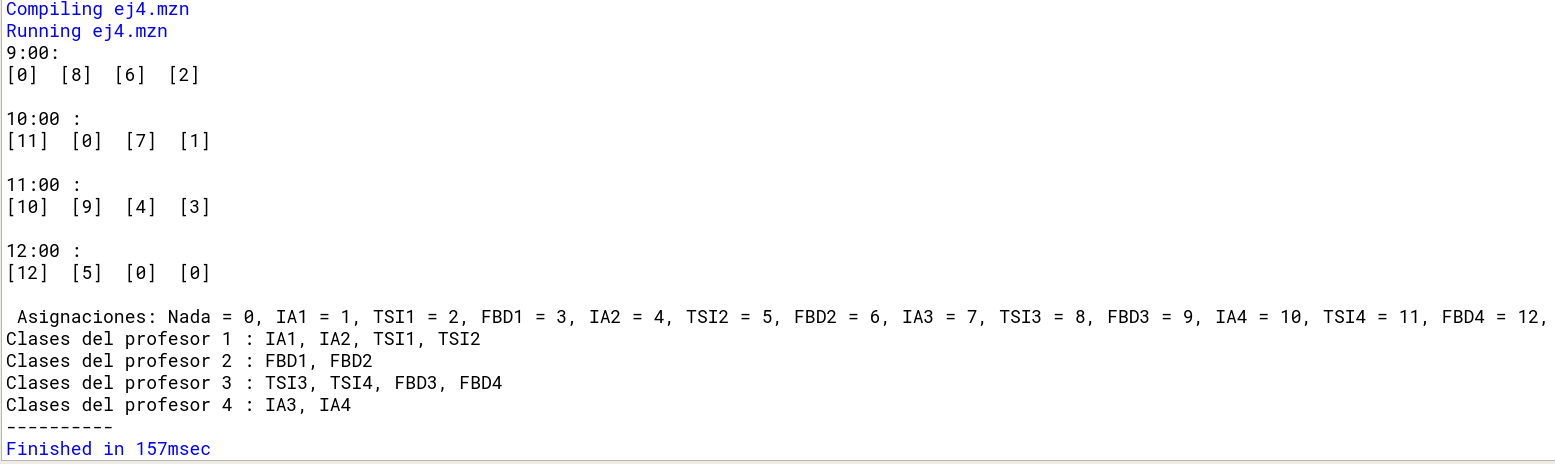
\includegraphics[scale = 0.30]{sol4.png}
 		 \caption{Solución obtenida para el ejercicio 4.}
  		\label{fig:ej4}

\end{figure}

\section{Ejercicio 5}

\subsection{Variables}

\subsection{Dominio de las variables}

\subsection{Restricciones}

\subsection{Resultado}


\begin{figure}[H]
  \centering
      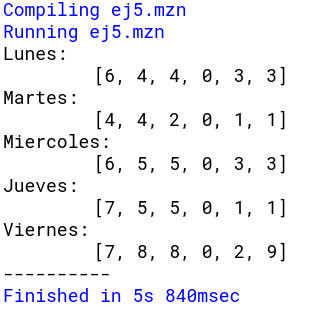
\includegraphics[scale = 0.30]{sol5.png}
 		 \caption{Solución obtenida para el ejercicio 5.}
  		\label{fig:ej5}

\end{figure}


\section{Ejercicio 6}

\subsection{Variables}

\subsection{Dominio de las variables}

\subsection{Restricciones}

\subsection{Resultado}


\begin{figure}[H]
  \centering
      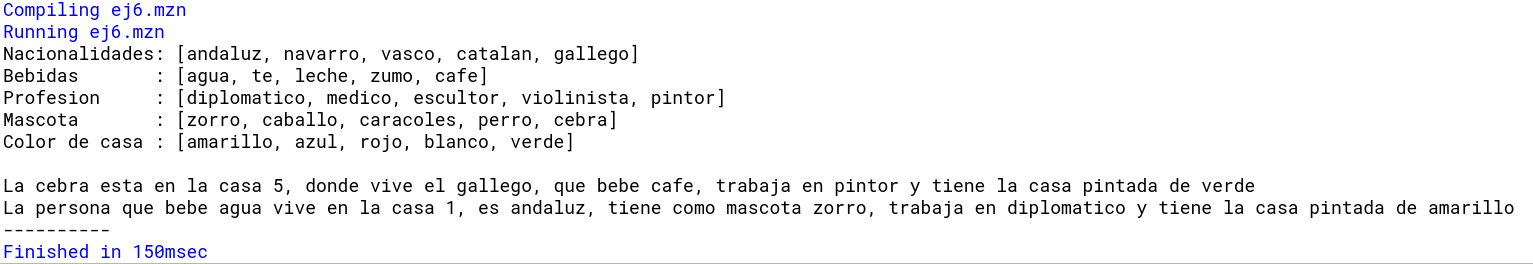
\includegraphics[scale = 0.30]{sol6.png}
 		 \caption{Solución obtenida para el ejercicio 6.}
  		\label{fig:ej6}

\end{figure}

\section{Ejercicio 7}

\subsection{Variables}

\subsection{Dominio de las variables}

\subsection{Restricciones}

\subsection{Resultado}


\begin{figure}[H]
  \centering
      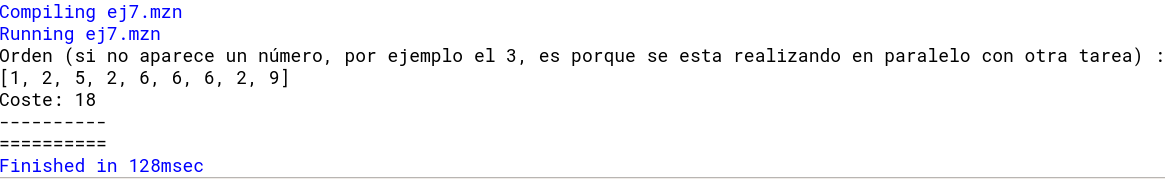
\includegraphics[scale = 0.30]{sol7.png}
 		 \caption{Solución obtenida para el ejercicio 7.}
  		\label{fig:ej7}

\end{figure}


%\section{Ejercicio 8}

%\subsection{Variables}

%\subsection{Dominio de las variables}

%\subsection{Restricciones}

%\subsection{Resultado}


%\section{Ejercicio 9}

%\subsection{Variables}

%\subsection{Dominio de las variables}

%\subsection{Restricciones}

%\subsection{Resultado}



\section{Ejercicio 10}

\subsection{Variables}

\subsection{Dominio de las variables}

\subsection{Restricciones}

\subsection{Resultado}


\begin{figure}[H]
  \centering
      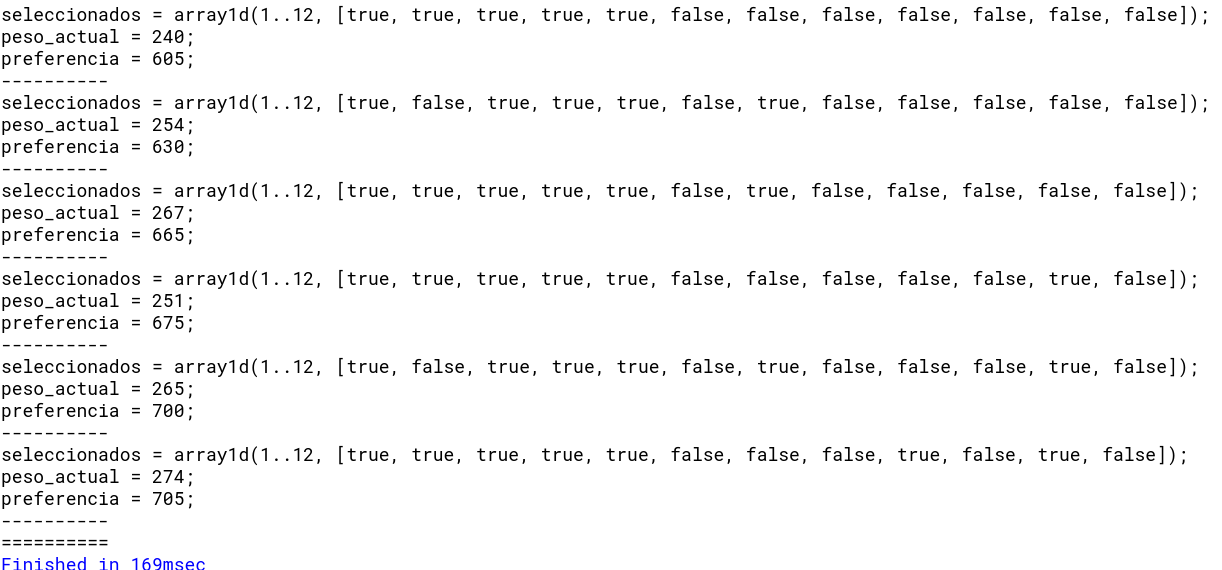
\includegraphics[scale = 0.30]{sol10.png}
 		 \caption{Solución obtenida para el ejercicio 10.}
  		\label{fig:ej10}

\end{figure}


\end{document}
